\documentclass[aspectratio=169,10pt,t]{beamer}
% \usetheme[
% %%% options passed to the outer theme
% %    progressstyle=fixedCircCnt,   %either fixedCircCnt, movCircCnt, or corner
% %    rotationcw,          % change the rotation direction from counter-clockwise to clockwise
% %    shownavsym          % show the navigation symbols
%   ]{SDUsimple}
\usepackage{SDUtheme/beamerthemeSDUsimple}
% If you want to change the colors of the various elements in the theme, edit and uncomment the following lines
% Change the bar and sidebar colors:
%\setbeamercolor{SDUsimple}{fg=red!20,bg=red}
%\setbeamercolor{sidebar}{bg=red!20}
% Change the color of the structural elements:
%\setbeamercolor{structure}{fg=red}
% Change the frame title text color:
%\setbeamercolor{frametitle}{fg=blue}
% Change the normal text color background:
%\setbeamercolor{normal text}{fg=black,bg=gray!10}
% ... and you can of course change a lot more - see the beamer user manual.
\usepackage{color}
\usepackage{float}
\usepackage{dsfont}                         % Enables double stroke fonts
\usepackage{bm}
\usepackage[utf8]{inputenc}
\usepackage[english]{babel}
\usepackage[T1]{fontenc}
\usepackage{listings}
\usepackage{amsmath}
\usepackage{import}
% Or whatever. Note that the encoding and the font should match. If T1
% does not look nice, try deleting the line with the fontenc.
\usepackage{helvet}
\usefonttheme{professionalfonts}

\newtheorem{algorithm}{Algorithm}
%\newtheorem{problem}{Problem}
\newtheorem{proposition}{Proposition}
% colored hyperlinks
\newcommand{\chref}[2]{%
	\href{#1}{{\usebeamercolor[bg]{SDUsimple}#2}}%
}

\title{One and two sample hotelling T$^2$-test}
\subtitle{Multivariate Statistic}
%\date{\today}
\date{ }

\author{
	Made by: \\
	\textbf{Lasse Gøransson, Marc Evald, Anne-Charlotte Poulsen \& Aske Møller}
}

% - Give the names in the same order as they appear in the paper.
% - Use the \inst{?} command only if the authors have different
%   affiliation. See the beamer manual for an example

\institute[
%  {\includegraphics[scale=0.2]{SDU_segl}}\\ %insert a company, department or university logo
SDU Robotics\\
The Maersk Mc-Kinney Moller Institute\\
University of Southern Denmark
] % optional - is placed in the bottom of the sidebar on every slide
{% is placed on the bottom of the title page
	SDU Robotics\\
	The Maersk Mc-Kinney Moller Institute\\
	University of Southern Denmark

	%there must be an empty line above this line - otherwise some unwanted space is added between the university and the country (I do not know why;( )
}

% specify a logo on the titlepage (you can specify additional logos an include them in
% institute command below
\pgfdeclareimage[height=0.5cm]{titlepagelogo}{SDUgraphics/SDU_logo_new} % placed on the title page
%\pgfdeclareimage[height=1.5cm]{titlepagelogo2}{SDUgraphics/SDU_logo_new} % placed on the title page
\titlegraphic{% is placed on the bottom of the title page
	\pgfuseimage{titlepagelogo}
	%  \hspace{1cm}\pgfuseimage{titlepagelogo2}
}

\begin{document}
% the titlepage
{\SDUwavesbg%
	\begin{frame}[plain,noframenumbering] % the plain option removes the header from the title page
		\titlepage
\end{frame}}
%%%%%%%%%%%%%%%%

\begin{frame}[t]
	\frametitle{Agenda}
	\begin{itemize}
		\item Motivation
		\item One-sample
		\item Two-sample
		\item Bartlett
	\end{itemize} 
\end{frame}

\begin{frame}[t]
	\frametitle{Motivation}

	\\
	\vspace{1cm}
	\pause

	Assumptions 

	\begin{itemize}
		\item Obs. IID
		\item MVN distributed 
	\end{itemize}

\end{frame}

\begin{frame}{Hypothesis Testing on $\mu$}{One-sample}


	Hypothesis

	\begin{align*}
		H_0&: \mu = \mu_0\\
		H_1&: \mu \neq \mu_0
	\end{align*}

	\begin{align*}
		T^2_0 = ( \bar{x} - \mu_0) \left(\frac{S^2}{n}\right)^{-1} ( \bar{x} -\mu_0 ) \sim \frac{p(n-1)}{n-p} F_{p,n-p}
	\end{align*}

\end{frame}

\begin{frame}{Hypothesis Testing on $\mu$}{One-sample}
	Hypothesis

	\begin{align*}
		H_0&: \mu = \mu_0\\
		H_1&: \mu \neq \mu_0
	\end{align*}

	\begin{align*}
		T^2_0 = ( \bar{X} - \mu_0) \left(\frac{S^2}{n}\right)^{-1} ( \bar{X} -\mu_0 ) \sim \frac{p(n-1)}{n-p} F_{p,n-p}
	\end{align*}

	\begin{columns}
		\begin{column}{0.5\textwidth}
			\begin{align*}
				t^2_0 > \frac{p(n-1)}{n-p} F_{p,n-p,\alpha } \\
				\text{Reject}
			\end{align*}
		\end{column}
		\begin{column}{0.5\textwidth}
			\begin{align*}
				P( F_{p,n-p} > \frac{n-p}{p(n-1)} t_0^2 )
			\end{align*}
		\end{column}
	\end{columns}



\end{frame}

\begin{frame}{Hypothesis Testing on $\mu$}{One-sample}
	\begin{figure}[H]
		\centering
		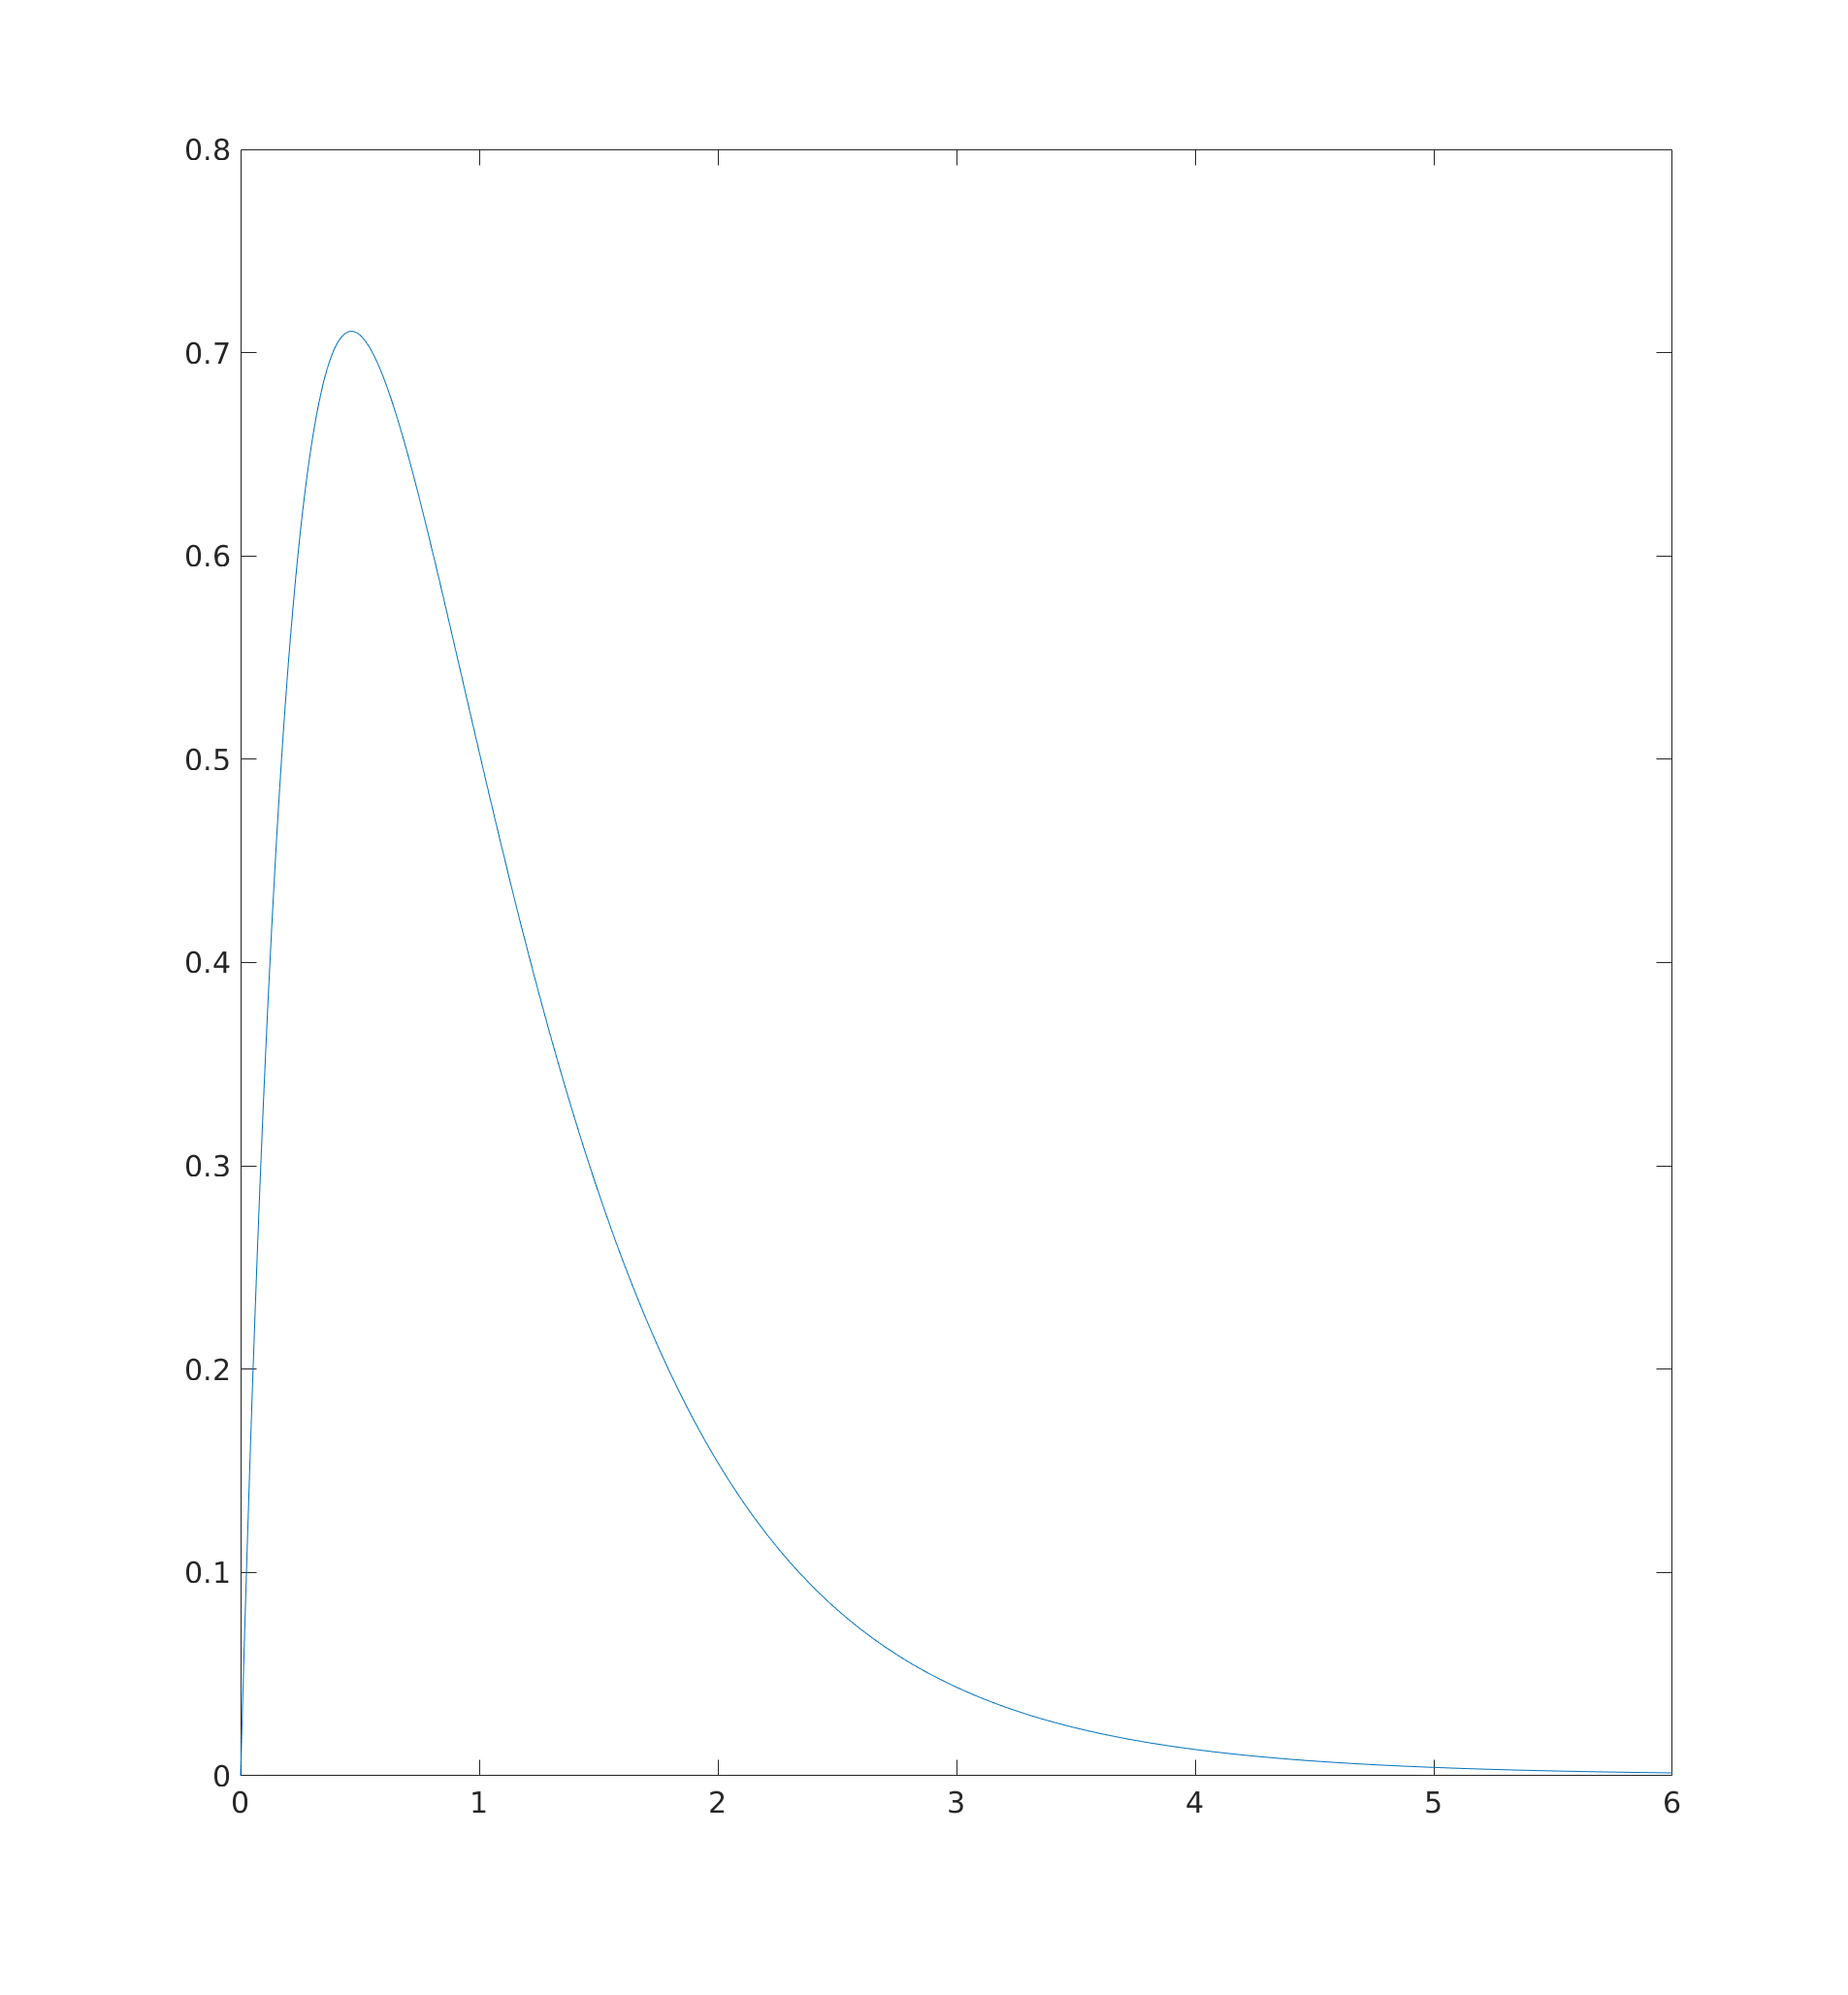
\includegraphics[scale=0.15]{images/f.png}
	\end{figure} 
\end{frame}

\begin{frame}[t]
	\frametitle{Motivation}

\end{frame}

\begin{frame}{Hypothesis Testing on $\mu$}{Two-sample}

	Assumptions.

	Model:
	\begin{itemize}
		\item Pair wise observations. $X$ and $Y$.
	\end{itemize}
	\\
	Difference model:
	\begin{itemize}
		\item 
			$ D =   \left( X - Y  \right)  \sim N \left( \mu_D, \Sigma_D  \right)  $
	\end{itemize}

	Hypothesis
	\begin{align*}
		H_0&: \mu_D = \delta\\
		H_1&: \mu_D \neq \delta
	\end{align*}

\end{frame}

\begin{frame}{Hypothesis Testing}{Paired comparison}
	Estimates: \\
	\begin{itemize}
		\item $\bar{D} = \frac{1}{n} \sum^n_{j=1} D_j$ 
		\item $S_d = \frac{1}{n-1} \sum^n_{j=1} \left(D_j - \bar{D} \right)^T \left(D_j - \bar{D} \right)$ 
	\end{itemize}
	Test Statistic: \\
	\begin{center}
		\quad $T_0^2 = \left( \bar{D} - \delta_0 \right)^T \left( \frac{S_d}{n}  \right) ^{-1} \left( \bar{D} - \delta_0 \right)$ \\
	\end{center}
	Reject: \\
	\begin{itemize}
		\item p-value
		\item Critical value
	\end{itemize}
\end{frame}

\begin{frame}[t]
	\frametitle{Hypothesis Testing on $\mu$}
	\framesubtitle{Equal $\Sigma$}
	\begin{itemize}
		\item Equal $\Sigma$\\
			\[
				S_p = 
				\frac{  \left( n_1 -1  \right) S_1 +  \left( n_2 -1  \right) S_2}
				{ \left( n_1 -1  \right) +  \left( n_2 -1  \right) } 
			\] 
		\item Unequal $\Sigma$
			\[
				T^{2} =
				\left( \bar{D} - \delta  \right) ^{T}
				\left( \frac{S_1}{n_1} + \frac{S_2}{n_2}  \right) ^{-1}
				\left( \bar{D} - \delta  \right)
			\] 
	\end{itemize}
\end{frame}
\begin{frame}[t]
	\frametitle{Confidence regions}
	\framesubtitle{subtitle}
	Confidence region for $\delta$
	\[
		\forall \delta \in {\rm I\!R}^{P}:
		\left( \bar{D} - \delta  \right) ^{T}
		\left( \frac{S_d}{n}  \right) ^{-1}
		\left( \bar{D} - \delta  \right)
		<
		\frac{p  \left( n-1 \right) }{n-p} 
		F_{p,n-p,\alpha}
	\] 
	\begin{figure}[h]
		\centering
		\import{../01/images/}{mvn.pdf_tex}
	\end{figure}
\end{frame}

\begin{frame}[t]
	\frametitle{Bartlett test}
	\framesubtitle{subtitle}
	Hypothesis:
	\[
		\begin{aligned}
			H_0 &: \Sigma_X = \Sigma_Y\\
			H_1 &: \Sigma_X \neq \Sigma_Y
		\end{aligned}
	\] 

	\[
		\begin{aligned}
			\Lambda &= \frac{
				\underset{\Sigma}{max}L \left( \Sigma \right) 
				}{
				\underset{\Sigma_X,\Sigma_Y}{max}L  \left( \Sigma_X,\Sigma_Y  \right) 
			} \\
			-2 \log  \Lambda
	&\approx
	\left( n_{X} + n_{Y} -2  \right) \cdot \log  |S_{p}| 
	-  \left( n_{X} -1  \right) \cdot \log |S_{X}|
	-  \left( n_{Y} -1  \right) \cdot \log |S_{Y}|\\
	-2 \log  \Lambda
	& \underset{approx}{\sim}
	\chi^{2}_{p \frac{p+1}{2} }
	\end{aligned}
\] 

\end{frame}

\end{document}
